\documentclass[12pt]{article}
\usepackage[margin=1in]{geometry}
\usepackage[utf8]{inputenc}
\usepackage[T1]{fontenc}
\usepackage{amsmath}
\usepackage{pgfplots}
\pgfplotsset{compat=1.17}
\usepackage{enumitem}

\begin{document}

% --- QUESTION 1 ---
\section*{FRQ 3 Practice: The Ferris Wheel}
The ``Sky Eye'' Ferris wheel is rotating at a constant speed. At time $t=0$ minutes, a rider boards a passenger car at the bottom of the wheel, which is 10 feet above the ground ($h(0)=10$). As the wheel turns, the rider reaches a maximum height of 110 feet above the ground. The wheel completes 3 full revolutions in 45 minutes. The sinusoidal function $h$ models the rider's height above the ground in feet as a function of time $t$ in minutes, for $0 \le t \le 45$.

\subsection*{(A)}
The graph of $h$ and its dashed midline for two full cycles is shown. Determine possible coordinates $(t, h(t))$ for the five points: F, G, J, K, and P.

\begin{center}
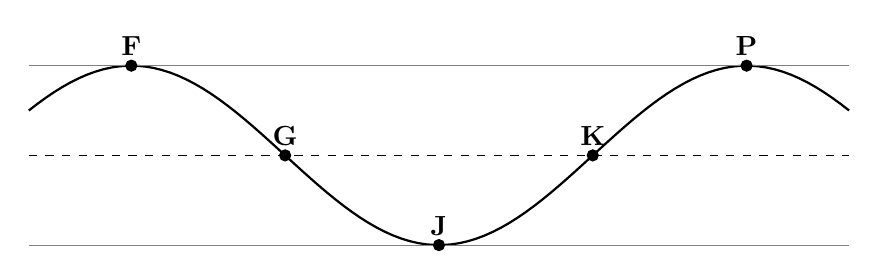
\begin{tikzpicture}
\begin{axis}[width=12cm, height=5cm, axis lines=none, xmin=5, xmax=25, ymin=-1.5, ymax=1.5, clip=false]
    \draw[dashed, black] (axis cs: 5, 0) -- (axis cs: 25, 0);
    \addplot[thick, domain=5:25, samples=100] {cos(deg(2*pi/15 * (x - 7.5)))};
    \addplot[mark=*, mark size=2pt] coordinates {(7.5, 1)}; \node[above] at (axis cs: 7.5, 1) {\textbf{F}};
    \addplot[mark=*, mark size=2pt] coordinates {(11.25, 0)}; \node[above] at (axis cs: 11.25, 0) {\textbf{G}};
    \addplot[mark=*, mark size=2pt] coordinates {(15, -1)}; \node[above] at (axis cs: 15, -1) {\textbf{J}};
    \addplot[mark=*, mark size=2pt] coordinates {(18.75, 0)}; \node[above] at (axis cs: 18.75, 0) {\textbf{K}};
    \addplot[mark=*, mark size=2pt] coordinates {(22.5, 1)}; \node[above] at (axis cs: 22.5, 1) {\textbf{P}};
    \draw[gray, thin] (axis cs: 5, 1) -- (axis cs: 25, 1); \draw[gray, thin] (axis cs: 5, -1) -- (axis cs: 25, -1);
\end{axis}
\end{tikzpicture}
\end{center}

\begin{itemize}[label={}]
    \item $F(\underline{\hspace{2cm}}, \underline{\hspace{2cm}}) \quad G(\underline{\hspace{2cm}}, \underline{\hspace{2cm}}) \quad J(\underline{\hspace{2cm}}, \underline{\hspace{2cm}})$
    \item $K(\underline{\hspace{2cm}}, \underline{\hspace{2cm}}) \quad P(\underline{\hspace{2cm}}, \underline{\hspace{2cm}})$
\end{itemize}

\subsection*{(B)}
The function $h$ can be written in the form $h(t) = a \cos(b(t+c)) + d$. Find constants $a, b, c, d$.

\vspace{0.5em}
$a = \underline{\hspace{1.5cm}} \quad b = \underline{\hspace{1.5cm}} \quad c = \underline{\hspace{1.5cm}} \quad d = \underline{\hspace{1.5cm}}$

\subsection*{(C)}
Refer to the graph of $h$ in part (A). The $t$-coordinate of G is $t_1$, and J is $t_2$.
(i) On the interval $(t_1, t_2)$, which is true about $h$?
\begin{enumerate}[label=\alph*.]
    \item $h$ is positive and increasing. \hfill b. $h$ is positive and decreasing.
    \item $h$ is negative and increasing. \hfill d. $h$ is negative and decreasing.
\end{enumerate}
(ii) Describe how the rate of change of $h$ is changing on the interval $(t_1, t_2)$.
\vspace{1.5cm}

\newpage
\section*{Solution 1}
\textbf{(A)} F(7.5, 110), G(11.25, 60), J(15, 10), K(18.75, 60), P(22.5, 110) \\
\textbf{(B)} $a = 50, \quad b = \frac{2\pi}{15}, \quad c = -7.5, \quad d = 60$ \\
\textbf{(C)} (i) b. (ii) Rate of change is \textbf{increasing} (concave up).

\newpage

% --- QUESTION 2 ---
\section*{FRQ 3 Practice: The Tides}
A pier piling is partially submerged. At $t=0$ hours, it is high tide, depth 18 feet ($h(0)=18$). The depth decreases to low tide at $t=6$ hours (depth 6 feet). The cycle repeats continuously.

\subsection*{(A)}
The graph of $h$ is shown. Determine coordinates for F, G, J, K, and P.

\begin{center}
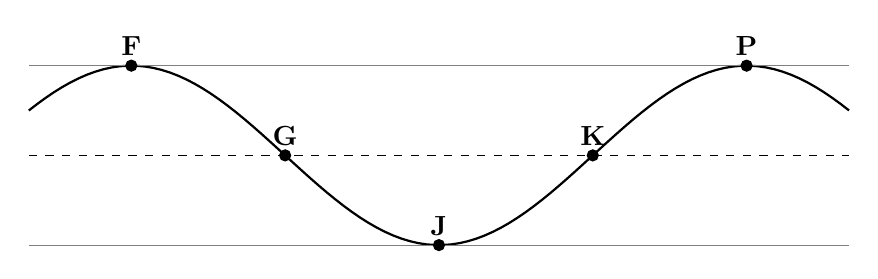
\begin{tikzpicture}
\begin{axis}[width=12cm, height=5cm, axis lines=none, xmin=-2, xmax=14, ymin=-1.5, ymax=1.5, clip=false]
    \draw[dashed, black] (axis cs: -2, 0) -- (axis cs: 14, 0);
    \addplot[thick, domain=-2:14, samples=100] {cos(deg(2*pi/12 * (x - 0)))};
    \addplot[mark=*, mark size=2pt] coordinates {(0, 1)}; \node[above] at (axis cs: 0, 1) {\textbf{F}};
    \addplot[mark=*, mark size=2pt] coordinates {(3, 0)}; \node[above] at (axis cs: 3, 0) {\textbf{G}};
    \addplot[mark=*, mark size=2pt] coordinates {(6, -1)}; \node[above] at (axis cs: 6, -1) {\textbf{J}};
    \addplot[mark=*, mark size=2pt] coordinates {(9, 0)}; \node[above] at (axis cs: 9, 0) {\textbf{K}};
    \addplot[mark=*, mark size=2pt] coordinates {(12, 1)}; \node[above] at (axis cs: 12, 1) {\textbf{P}};
    \draw[gray, thin] (axis cs: -2, 1) -- (axis cs: 14, 1); \draw[gray, thin] (axis cs: -2, -1) -- (axis cs: 14, -1);
\end{axis}
\end{tikzpicture}
\end{center}

\begin{itemize}[label={}]
    \item $F(\underline{\hspace{2cm}}, \underline{\hspace{2cm}}) \quad G(\underline{\hspace{2cm}}, \underline{\hspace{2cm}}) \quad J(\underline{\hspace{2cm}}, \underline{\hspace{2cm}})$
    \item $K(\underline{\hspace{2cm}}, \underline{\hspace{2cm}}) \quad P(\underline{\hspace{2cm}}, \underline{\hspace{2cm}})$
\end{itemize}

\subsection*{(B)}
Find constants $a, b, c, d$ for $h(t) = a \cos(b(t+c)) + d$.

\vspace{0.5em}
$a = \underline{\hspace{1.5cm}} \quad b = \underline{\hspace{1.5cm}} \quad c = \underline{\hspace{1.5cm}} \quad d = \underline{\hspace{1.5cm}}$

\subsection*{(C)}
Refer to graph in (A). $t$-coord of J is $t_1$, K is $t_2$.
(i) On interval $(t_1, t_2)$, which is true?
\begin{enumerate}[label=\alph*.]
    \item $h$ is positive and increasing. \hfill b. $h$ is positive and decreasing.
    \item $h$ is negative and increasing. \hfill d. $h$ is negative and decreasing.
\end{enumerate}
(ii) Describe how the rate of change of $h$ is changing on $(t_1, t_2)$.
\vspace{1.5cm}

\newpage
\section*{Solution 2}
\textbf{(A)} F(0, 18), G(3, 12), J(6, 6), K(9, 12), P(12, 18) \\
\textbf{(B)} $a = 6, \quad b = \frac{\pi}{6}, \quad c = 0, \quad d = 12$ \\
\textbf{(C)} (i) a. (ii) Rate of change is \textbf{increasing} (concave up).

\newpage

% --- QUESTION 3 ---
\section*{FRQ 3 Practice: The Pendulum}
A hypnosis pendulum swings. At $t=0$, the bob is at its furthest point right, 8 cm from center ($h(0)=8$). It swings left to -8 cm, then returns. It completes 5 full swings in 10 seconds.

\subsection*{(A)}
The graph of $h$ is shown. Determine coordinates for F, G, J, K, and P.

\begin{center}
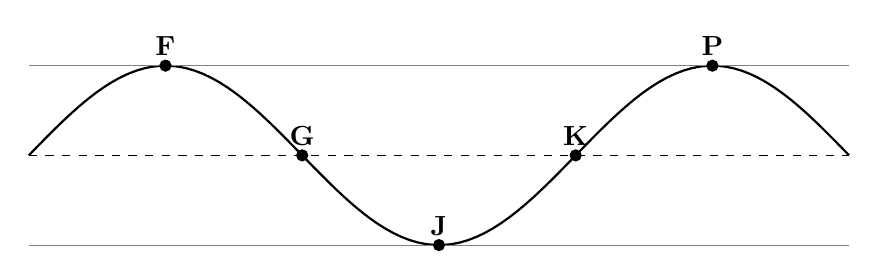
\begin{tikzpicture}
\begin{axis}[width=12cm, height=5cm, axis lines=none, xmin=-0.5, xmax=2.5, ymin=-1.5, ymax=1.5, clip=false]
    \draw[dashed, black] (axis cs: -0.5, 0) -- (axis cs: 2.5, 0);
    \addplot[thick, domain=-0.5:2.5, samples=100] {cos(deg(2*pi/2 * (x - 0)))};
    \addplot[mark=*, mark size=2pt] coordinates {(0, 1)}; \node[above] at (axis cs: 0, 1) {\textbf{F}};
    \addplot[mark=*, mark size=2pt] coordinates {(0.5, 0)}; \node[above] at (axis cs: 0.5, 0) {\textbf{G}};
    \addplot[mark=*, mark size=2pt] coordinates {(1.0, -1)}; \node[above] at (axis cs: 1.0, -1) {\textbf{J}};
    \addplot[mark=*, mark size=2pt] coordinates {(1.5, 0)}; \node[above] at (axis cs: 1.5, 0) {\textbf{K}};
    \addplot[mark=*, mark size=2pt] coordinates {(2.0, 1)}; \node[above] at (axis cs: 2.0, 1) {\textbf{P}};
    \draw[gray, thin] (axis cs: -0.5, 1) -- (axis cs: 2.5, 1); \draw[gray, thin] (axis cs: -0.5, -1) -- (axis cs: 2.5, -1);
\end{axis}
\end{tikzpicture}
\end{center}

\begin{itemize}[label={}]
    \item $F(\underline{\hspace{2cm}}, \underline{\hspace{2cm}}) \quad G(\underline{\hspace{2cm}}, \underline{\hspace{2cm}}) \quad J(\underline{\hspace{2cm}}, \underline{\hspace{2cm}})$
    \item $K(\underline{\hspace{2cm}}, \underline{\hspace{2cm}}) \quad P(\underline{\hspace{2cm}}, \underline{\hspace{2cm}})$
\end{itemize}

\subsection*{(B)}
Find constants $a, b, c, d$ for $h(t) = a \cos(b(t+c)) + d$.

\vspace{0.5em}
$a = \underline{\hspace{1.5cm}} \quad b = \underline{\hspace{1.5cm}} \quad c = \underline{\hspace{1.5cm}} \quad d = \underline{\hspace{1.5cm}}$

\subsection*{(C)}
Refer to graph in (A). $t$-coord of F is $t_1$, G is $t_2$.
(i) On interval $(t_1, t_2)$, which is true?
\begin{enumerate}[label=\alph*.]
    \item $h$ is positive and increasing. \hfill b. $h$ is positive and decreasing.
    \item $h$ is negative and increasing. \hfill d. $h$ is negative and decreasing.
\end{enumerate}
(ii) Describe how the rate of change of $h$ is changing on $(t_1, t_2)$.
\vspace{1.5cm}

\newpage
\section*{Solution 3}
\textbf{(A)} F(0, 8), G(0.5, 0), J(1.0, -8), K(1.5, 0), P(2.0, 8) \\
\textbf{(B)} $a = 8, \quad b = \pi, \quad c = 0, \quad d = 0$ \\
\textbf{(C)} (i) b. (ii) Rate of change is \textbf{decreasing} (concave down).

\newpage

% --- QUESTION 4 ---
\section*{FRQ 3 Practice: The Reptile Heater}
A reptile heater cycles. At $t=0$, it starts at average $80^\circ$F and rises. Max is $95^\circ$F, Min is $65^\circ$F. Cycle repeats every 8 hours.

\subsection*{(A)}
The graph of $h$ is shown. Determine coordinates for F, G, J, K, and P.

\begin{center}
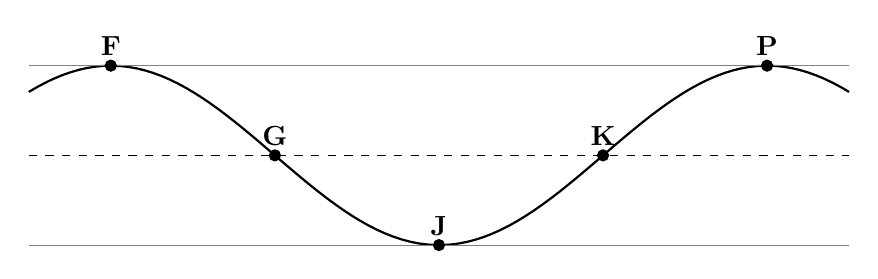
\begin{tikzpicture}
\begin{axis}[width=12cm, height=5cm, axis lines=none, xmin=1, xmax=11, ymin=-1.5, ymax=1.5, clip=false]
    \draw[dashed, black] (axis cs: 1, 0) -- (axis cs: 11, 0);
    \addplot[thick, domain=1:11, samples=100] {cos(deg(2*pi/8 * (x - 2)))};
    \addplot[mark=*, mark size=2pt] coordinates {(2, 1)}; \node[above] at (axis cs: 2, 1) {\textbf{F}};
    \addplot[mark=*, mark size=2pt] coordinates {(4, 0)}; \node[above] at (axis cs: 4, 0) {\textbf{G}};
    \addplot[mark=*, mark size=2pt] coordinates {(6, -1)}; \node[above] at (axis cs: 6, -1) {\textbf{J}};
    \addplot[mark=*, mark size=2pt] coordinates {(8, 0)}; \node[above] at (axis cs: 8, 0) {\textbf{K}};
    \addplot[mark=*, mark size=2pt] coordinates {(10, 1)}; \node[above] at (axis cs: 10, 1) {\textbf{P}};
    \draw[gray, thin] (axis cs: 1, 1) -- (axis cs: 11, 1); \draw[gray, thin] (axis cs: 1, -1) -- (axis cs: 11, -1);
\end{axis}
\end{tikzpicture}
\end{center}

\begin{itemize}[label={}]
    \item $F(\underline{\hspace{2cm}}, \underline{\hspace{2cm}}) \quad G(\underline{\hspace{2cm}}, \underline{\hspace{2cm}}) \quad J(\underline{\hspace{2cm}}, \underline{\hspace{2cm}})$
    \item $K(\underline{\hspace{2cm}}, \underline{\hspace{2cm}}) \quad P(\underline{\hspace{2cm}}, \underline{\hspace{2cm}})$
\end{itemize}

\subsection*{(B)}
Find constants $a, b, c, d$ for $h(t) = a \sin(b(t+c)) + d$.

\vspace{0.5em}
$a = \underline{\hspace{1.5cm}} \quad b = \underline{\hspace{1.5cm}} \quad c = \underline{\hspace{1.5cm}} \quad d = \underline{\hspace{1.5cm}}$

\subsection*{(C)}
Refer to graph in (A). $t$-coord of G is $t_1$, J is $t_2$.
(i) On interval $(t_1, t_2)$, which is true?
\begin{enumerate}[label=\alph*.]
    \item $h$ is positive and increasing. \hfill b. $h$ is positive and decreasing.
    \item $h$ is negative and increasing. \hfill d. $h$ is negative and decreasing.
\end{enumerate}
(ii) Describe how the rate of change of $h$ is changing on $(t_1, t_2)$.
\vspace{1.5cm}

\newpage
\section*{Solution 4}
\textbf{(A)} F(2, 95), G(4, 80), J(6, 65), K(8, 80), P(10, 95) \\
\textbf{(B)} $a = 15, \quad b = \frac{\pi}{4}, \quad c = 0, \quad d = 80$ \\
\textbf{(C)} (i) b. (ii) Rate of change is \textbf{increasing} (concave up).

\newpage

% --- QUESTION 5 ---
\section*{FRQ 3 Practice: The Ocean Buoy}
A buoy bobbing in waves starts at min ($t=0, h=-3$), rises to max ($3$ ft), then drops. Cycle is 6 seconds.

\subsection*{(A)}
The graph of $h$ is shown. Determine coordinates for F, G, J, K, and P.

\begin{center}
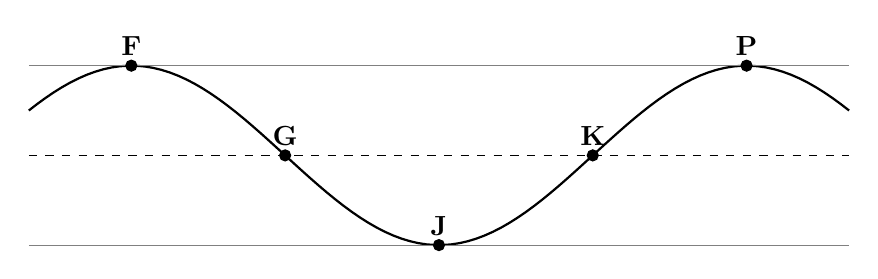
\begin{tikzpicture}
\begin{axis}[width=12cm, height=5cm, axis lines=none, xmin=2, xmax=10, ymin=-1.5, ymax=1.5, clip=false]
    \draw[dashed, black] (axis cs: 2, 0) -- (axis cs: 10, 0);
    \addplot[thick, domain=2:10, samples=100] {cos(deg(2*pi/6 * (x - 3)))};
    \addplot[mark=*, mark size=2pt] coordinates {(3, 1)}; \node[above] at (axis cs: 3, 1) {\textbf{F}};
    \addplot[mark=*, mark size=2pt] coordinates {(4.5, 0)}; \node[above] at (axis cs: 4.5, 0) {\textbf{G}};
    \addplot[mark=*, mark size=2pt] coordinates {(6, -1)}; \node[above] at (axis cs: 6, -1) {\textbf{J}};
    \addplot[mark=*, mark size=2pt] coordinates {(7.5, 0)}; \node[above] at (axis cs: 7.5, 0) {\textbf{K}};
    \addplot[mark=*, mark size=2pt] coordinates {(9, 1)}; \node[above] at (axis cs: 9, 1) {\textbf{P}};
    \draw[gray, thin] (axis cs: 2, 1) -- (axis cs: 10, 1); \draw[gray, thin] (axis cs: 2, -1) -- (axis cs: 10, -1);
\end{axis}
\end{tikzpicture}
\end{center}

\begin{itemize}[label={}]
    \item $F(\underline{\hspace{2cm}}, \underline{\hspace{2cm}}) \quad G(\underline{\hspace{2cm}}, \underline{\hspace{2cm}}) \quad J(\underline{\hspace{2cm}}, \underline{\hspace{2cm}})$
    \item $K(\underline{\hspace{2cm}}, \underline{\hspace{2cm}}) \quad P(\underline{\hspace{2cm}}, \underline{\hspace{2cm}})$
\end{itemize}

\subsection*{(B)}
Find constants $a, b, c, d$ for $h(t) = a \cos(b(t+c)) + d$.

\vspace{0.5em}
$a = \underline{\hspace{1.5cm}} \quad b = \underline{\hspace{1.5cm}} \quad c = \underline{\hspace{1.5cm}} \quad d = \underline{\hspace{1.5cm}}$

\subsection*{(C)}
Refer to graph in (A). $t$-coord of K is $t_1$, P is $t_2$.
(i) On interval $(t_1, t_2)$, which is true?
\begin{enumerate}[label=\alph*.]
    \item $h$ is positive and increasing. \hfill b. $h$ is positive and decreasing.
    \item $h$ is negative and increasing. \hfill d. $h$ is negative and decreasing.
\end{enumerate}
(ii) Describe how the rate of change of $h$ is changing on $(t_1, t_2)$.
\vspace{1.5cm}

\newpage
\section*{Solution 5}
\textbf{(A)} F(3, 3), G(4.5, 0), J(6, -3), K(7.5, 0), P(9, 3) \\
\textbf{(B)} $a = 3, \quad b = \frac{\pi}{3}, \quad c = -3, \quad d = 0$ \\
\textbf{(C)} (i) a. (ii) Rate of change is \textbf{decreasing} (concave down).

\end{document}